% You should title the file with a .tex extension (hw1.tex, for example)
\documentclass[11pt]{article}

\usepackage{amsmath}
\usepackage{amssymb, qtree}
\usepackage{fancyhdr}
\usepackage{verbatim}
\usepackage{tikz}
\usepackage{algorithm2e}
\usepackage{graphicx}
\usepackage{mathtools}


\oddsidemargin0cm
\topmargin-2cm     %I recommend adding these three lines to increase the 
\textwidth16.5cm   %amount of usable space on the page (and save trees)
\textheight23.5cm  

\newcommand{\question}[2] {\vspace{.25in} \hrule\vspace{0.5em}
\noindent{\bf #1: #2} \vspace{0.5em}
\hrule \vspace{.10in}}
\renewcommand{\part}[1] {\vspace{.10in} {\bf (#1)}}

\newcommand{\myname}{Nitesh Turaga}
\newcommand{\myandrew}{nturaga@andrew.cmu.edu}
\newcommand{\myhwnum}{}

\setlength{\parindent}{0pt}
\setlength{\parskip}{5pt plus 1pt}
 
\pagestyle{fancyplain}
\lhead{\fancyplain{}{\textbf{\myhwnum}}}      % Note the different brackets!
\rhead{\fancyplain{}{\myname\\ \myandrew}}
\chead{\fancyplain{}{}}

\begin{document}

\medskip                        % Skip a "medium" amount of space
                                % (latex determines what medium is)
                                % Also try: \bigskip, \littleskip

\thispagestyle{plain}
\begin{center}                  % Center the following lines
{\Large Analyst Training Program(ATP)-Coding Assessment \myhwnum} \\
\myname \\
\myandrew \\
{\today}\
\end{center}

References: 
\begin{verbatim}
1. Mathworks Documentation center.
2. http://www.broadinstitute.org/cancer/software/genepattern/
gp_guides/file-formats/sections/gct
3. Unix documentation
4. Machine Learning, Tom M. Mitchell
5. Data Mining for Genomics and Proteomics, Darius M. Dziuda.
\end{verbatim}


\question{1}{Analysis of Gene expression data}

{\bf 1)}

The approach was to create a temporary file which skipped the first two header lines in the GCT file. Then, MATLAB provides an {\tt importdata(filename)} function, which lets me create a struct from the data fields. The point of creating the temporary file is to not touch the original file, this is a design choice.

We could also use, matlab function {\tt importdata('gene\_ expr\_ 500x204.gct')} to open files interactively. Parsing the files as a text file would be wasteful as there are better file parsing languages like Python or Perl.

{ \bf 2)}

Run the function plotCode.m, and the three graphs will be generated.

\begin{itemize}

\item[•]a)


$Box plot$ of the $log2$ expression values of the first 20 samples.

The approach was to use the inbuilt box plot function in MATLAB. Convert  all the expression values of the first 20 columns(samples) into $log2$ values and pass it into $boxplot$. I label the axes and use the matlab grid option.

\item[•]b)

Raw expression values of the first 10 analytes vs the sample index.

I noticed that the coloring scheme used was $lines$, specified by the matlab colormap. I used that to make the graph. I used a for loop to go through 1 to 10 because it was more intuitive and seemed clearer. 

For each sample, I got the value of that row, and all of its columns to plot the raw expression values using the $lines$ colormap.

The other choice was to use the $gscatter$ function in matlab, I have the alternative code written in the file, but it is commented out. Since, it did not seem like good coding style, I did not use it. If the comment is removed, that will work.


\item[•]c)

Calibration plot of the raw expression of the first 10 analytes vs the analyte index.

Plot the raw gene expression values for the first 10 analytes(first 10 rows) for all the columns and color is cyan. Then make an errorbar where the points are $median$ values of the gene expression of each analyte and the error bar is of length equal to the standard deviation for gene expression of each analyte.

The specifics of the figure are also implemented,using errorbar $LineSpec$. Alternative code is given in a commented out region for the plot function.


\end{itemize}


\question{2}{Analysis of flow cytometry data}

The approach for analysis of the flow cytometry data, was to first replicate the histograms given. I wrote a script for this in matlab, called $analysis.m$.

The script allows me to parse the file $P8.gct$, utilizing the function I wrote in the previous question. I make modification to this function in the script. So, while running the function, have the $gctparse.m$, in the same folder. 

The script reproduces the graphs given in the question and also, plots the expression values with respect to the time. I plot it only for 2 particle RID's, but there is similarity among the others as well. 

The graph below describes, the varying signal intensity over time. 
On the x-axis, we have "time" where the signal intensity of the particle 105 is recorded. On the y-axis, the $log2(RP1)$ values.
Since, there is varying intensity overtime, we can say that the intensity of the particle drifts over time.
The intensity drift can be accounted for many factors in flow cytometry. Since, the same cell is not analyzed again for the flow cytometer, we can expect a varying amount of florescence in the next cell from the same sample and hence, there is a difference in intensity over time, but very small variation. The cytometer detects the particle, if it matches the property of the distribution. \\

Graph for particle RID=105,	similar to the one above, 

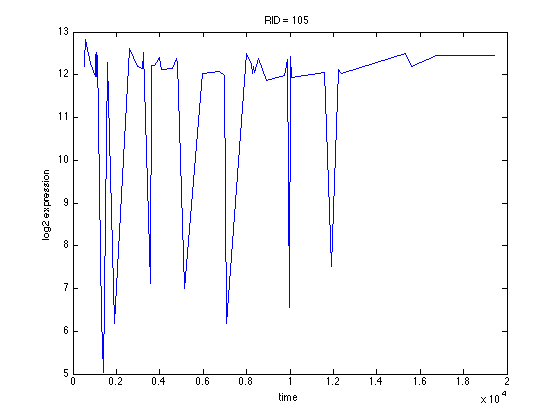
\includegraphics[scale=0.5]{rid105.png}



Graph for particle RID=401,	similar to the one above, 

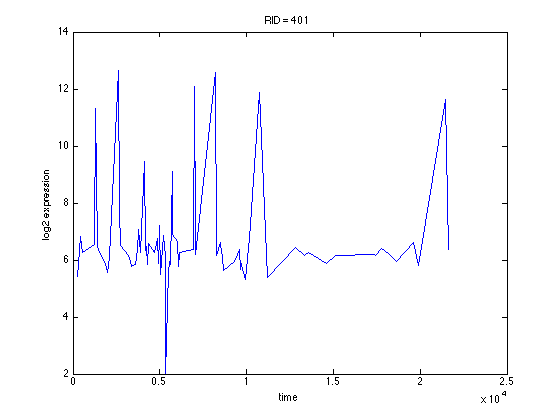
\includegraphics[scale=0.5]{rid401.png} 

NOTE:

A more ideal approach would be to analyze the instensity drift of all the particles over time. We could remove the outliers from the data for each particle RID. The approach would be to get the mean, and remove all the samples which are 1 standard deviation away from the mean on either side. If i re plot these leftover samples, the drift over time is very less.

{\bf As we can see the error is reduced and the drift over time also reduces greatly if the noise is removed. This allows the flow cytometer to classify particles better.} 



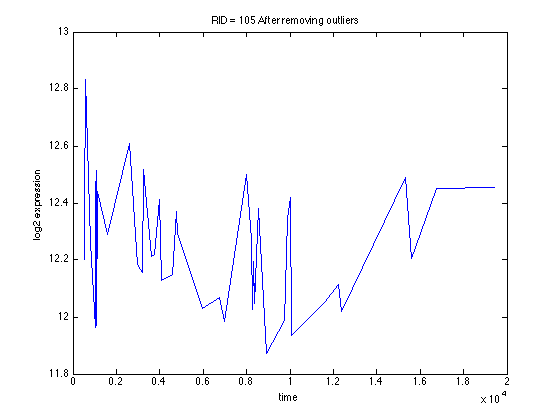
\includegraphics[scale=0.5]{105noOutliers.png}


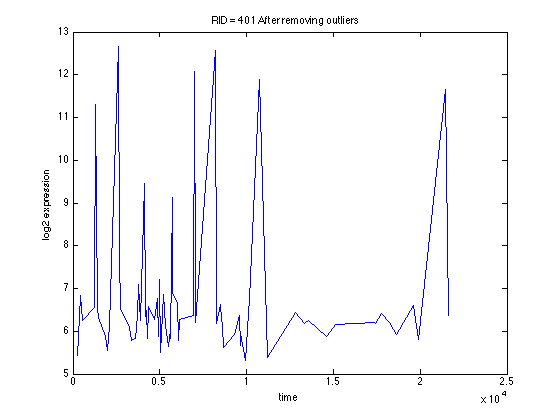
\includegraphics[scale=0.5]{401noOutliers.png}

\question{3}{Regression modeling of gene expression data}

\begin{enumerate}

\item{}

Approach:

I first use the $gctparse.m$ function I wrote in the first question to get the labels and the gene expression values into separate structures of the $train.gct$. The script $regressionModel.m$,call these functions. 

The next step was to separate the dependent from the predictor variables, let us call them, $remanining\_expr$ and $dependant\_expr$ respectively. $remaining\_expr$ has the size (979*2519) and $dependant\_expr$ has (21289*2519).  

The script gets the gene expression values of my $remaining\_expr$ and $dependent\_expr$ gene expressions. This could have easily done in unix, but the formatting of grep was introducing unforeseen errors(command: {\tt egrep -vf predictor.grp train.gct > dependentSet.gct}. 

The next step was to was to input the two matrices into the $regstats$ function inbuilt with MATLAB. This allows to get the coefficients of the function and also evaluate the training error of the model.



\item

Since, I used regstats in my function, the value of adjusted rsquared changes depending on the addition of variables, this is because adjusted rsquared is corrected for number of independent variables in the model.

Plot, can be generated by running the code.

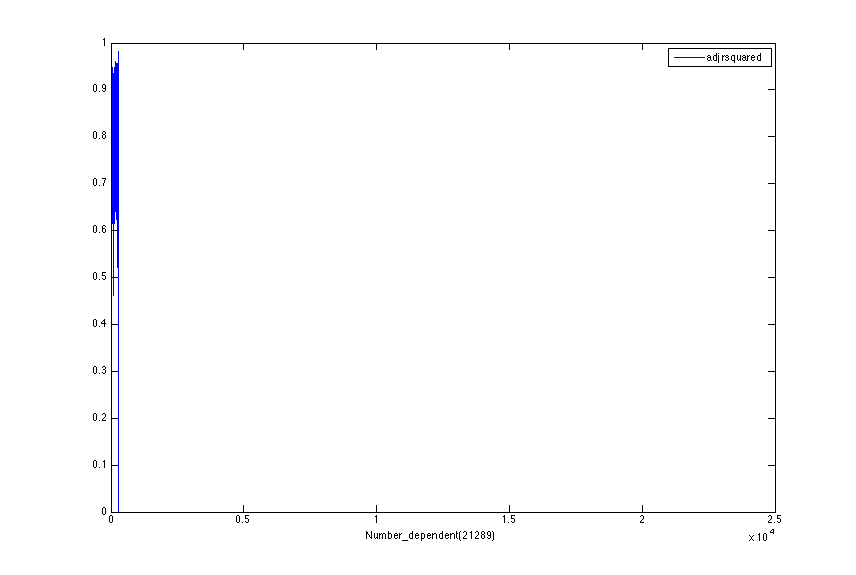
\includegraphics[scale=0.5]{sample300.png}

\item

Due to the running time being high, i reduced the size of the dependent variables and I used only a subset(300) of the remaining genes(predictor) to fit the model. The adjusted rsquared plotted does not make much sense, because the number of predicted genes is a lot.

But, to apply the model on the $test.gct$, I would have to use the coefficient values output, multiply it with the values of the test set and get the predicted $y$ value, from the multiple linear regression model.

But if the run for a long time, i believe that the model will work and will plot the adjusted rsquared values, and this can be applied to the test.gct to generate the required 22268*96 samples.



\end{enumerate}


\question{4}{Shell Scripting}

Souce code provided in $solution\_q4.txt$

{\bf 1)}
\begin{verbatim}
awk 'NR==3' gene_expr_500x204.gct |tr '\t' '\n' |tail -n +3 >samples.grp 

\end{verbatim}

{\tt awk 'NR==3' gene\_expr\_500x204.gct }; this command takes the third line of the GCT file which contain the sample names.

{\tt tr '\textbackslash t' '\textbackslash n'};this command piped with the previous one replaces the 'tab' delimiter between the sample names with 'newline' characters.

{\tt tail -n +3}; removes the words "Name" and "Desc" from the list.


{\bf NOTE:}

{\tt sed 's/\textasciicircum M//g'}; removes the \textasciicircum M character at the end of the file, which occurs because of unix to dos conversion. Use this only if that problem occurs on the machine. It is displayed sometimes on windows environments. In the event, add pipe after $tail$ and run.

I realize there are many other ways to do this.The whole thing can be done with only $awk$.

{\bf 2)}
\begin{verbatim}
awk {'printf ("%1c%02d\n",substr($1,1,1),substr($1,2,2))}'samples.grp|sort  >
 sorted_sample.grp
\end{verbatim}

The $awk$ command prints out 1 character , 2 digits and then a newline.$substr(\$1,1,1)$ represents the first character,$substr(\$1,2,2)$ represents the numbers after the character.

\begin{verbatim}
 "%1c%02d\n"; represents that each word has 1 char and 2 digits, and provides 
padding with a "0" before the 2 digits.And adds a newline after that.
\end{verbatim}


\end{document}

